\section{Experiment}
% \subsection{Datasets and Experiment Settings}

% \subsubsection{Datasets and Evaluation Metrics.}

% \subsubsection{Baselines.}

% \subsubsection{Implementation Details.}
% RM-R1~\citep{chen2025rm}
% RRM~\citep{guo2025reward}
% JudgeLRM~\citep{chen2025judgelrm}

% Reward modeling benchmark:

% RewardBench~\citep{rewardbench}
% RM-Bench~\citep{liu2025rmbench}
% FollowBench~\citep{followbench}
% InfoBench~\citep{infobench}
% IFBench~\citep{ifbench}
% PPE-IFEval~\citep{ppe}
% RewardBench2 \citep{malik2025rewardbench2}


% Policy Model benchmark:
% Follow \citep{viswanathan2025checklists}, use IF benchmarks
% IFEval~\citep{zhou2023instruction}, InFoBench~\citep{infobench}
% Healthbench/medical reward modeling benchmark

\subsection{Datasets and Experiment Settings}
\label{subsec:datasets-settings}

\noindent \textbf{Training data.}
We train both components of {\name}: the \emph{rubric generator} and the \emph{judge}, on the curated {\dataset} as presented in Sec.~\ref{sec:rubrics_gen}. Rubrics are produced with contrastive signals from chosen/rejected responses and filtered by preference–label consistency before use. Unless otherwise noted, we use the science-related slice of OpenRubrics to better match our domain study on HealthBench/medical evaluation.

\noindent \textbf{Backbone and variants.}
Both the rubric generator and the judge are fine-tuned from Qwen-3-8B (``{\name}-8B'') unless specified. At inference time, {\name} follows the two-stage process as detailed in Sec \ref{sec:rm_train}. We also report an ensemble variant, \textit{voting@5}, which aggregates five independently sampled judge trajectories by majority vote.

\noindent \textbf{Baselines.}
We compare {\name} against strong, same-scale white-box reward (judge) models: JudgeLRM-7B~\citep{chen2025judgelrm}, RRM-7B~\citep{guo2025reward}, and RM-R1-7B~\citep{chen2025rm}.
We also report larger RM-R1-14B~\citep{chen2025rm} and API judges for reference when available. To isolate the benefit of rubric-aware fine-tuning, we include naive {Qwen-3-8B (Rubric+Judge)} that directly prompts the base model to produce rubrics and then make judgments.

\noindent \textbf{Evaluation benchmarks and metrics.}
We evaluate {\name} as a pairwise reward model on popular reward-modeling benchmarks: \emph{RewardBench} (Chat, Chat-Hard)~\citep{rewardbench}, \emph{RM-Bench}~\citep{liu2025rmbench}, \emph{PPE-IFEval}~\citep{ppe}, \emph{FollowBench}~\citep{followbench}, \emph{InfoBench}~\citep{infobench}, \emph{IFBench}~\citep{ifbench}, and \emph{RewardBench2} (Precise-IF, Focus)~\citep{malik2025rewardbench2}. 
While \emph{FollowBench} and \emph{InfoBench} were originally designed to assess instruction-following capabilities of LLMs, we adapt them to pairwise evaluation settings by sampling two responses from the same model (Qwen-3-8B/14B), where one response adheres to all specified constraints and the other violates some of them. 
For the domain study we additionally report HealthBench/medical results. We follow each benchmark’s official splits and scoring rules, reporting accuracy, win-rate or other specific scores.

Due to space limits, additioanl implementation details are deferred to Appendix \ref{apd:implementation_details}. 

% \begin{table*}[!t]
% \centering
% \caption{Comparison of different judge and reward models across multiple benchmarks. 
% RewardBench2 reports results on Precise IF, and Focus dimensions. 
% Rubric API uses GPT-4.1-Mini, and Judge API uses Gemini-2.5-Flash-Lite. 
% Best results are highlighted in \textbf{bold}.
% }
% \label{tab:main_results}
% \resizebox{0.99\textwidth}{!}{%
% \begin{tabular}{l cc cccc c cc cc}
% \toprule
% \multirow{2.5}{*}{} 
% & \multicolumn{2}{c}{\bf RewardBench} 
% & \multicolumn{4}{c}{\bf IF Evaluation Benchmarks} 
% & \bf RM-Bench
% & \multicolumn{2}{c}{\bf RewardBench2}
% & \multirow{2.5}{*}{\bf HelpSteer3}
% & \multirow{2.5}{*}{\bf AVG} \\ 
% \cmidrule(lr){2-3}  \cmidrule(lr){4-7} \cmidrule(lr){8-8} \cmidrule(lr){9-10}
%                             & Chat & Chat Hard  & FollowBench   &   PPE-IFEval  &   InfoBench   &   IFBench     &    Chat        & Precise IF    &   Focus  &      &   \\ 
% \midrule
% \multicolumn{11}{l}{\it Black-box LLMs (For reference only)} \\
% \midrule
% Claude-3.5-Sonnet           & 96.4 & 74.0       & --            & 58.0          & --            & --            & 62.5           & 38.8          & 87.0     & --   & - \\
% API (Rubric+Judge)          & 79.6 & 79.2       & 83.2          & 61.0          & 82.2          & 66.2          & 80.6/73.6/49.6 & 42.5          & 79.6	    & 71.4 & 71.3 \\
% API (direct Judge)          & 89.6 & 71.2       & 81.7          & 59.2          & 72.9          & 60.4          & 89.7/73.3/38.7 & 13.2          & 63.4     & 70.3 & 64.9 \\ 
% \midrule
% \multicolumn{11}{l}{\it Larger White-box LLMs (For reference only)} \\
% \midrule
% RM-R1-14B (Qwen-2.5-Inst)   & 73.5 & 79.8	    & 84.0	        & 59.0          & 85.5	        & 60.8          & 93.3/77.5/48.8 & 23.8	         & 84.6	    & 74.8 & 69.9 \\
% RM-R1-14B (DeepSeek-Dist)   & 90.3 & 78.9       & 89.9          & 61.2          & 82.4          & 59.0          & 90.2/77.3/46.8 & 30.6          & 79.0     & 74.6 & 71.7 \\
% \midrule
% \multicolumn{11}{l}{\it White-box Judge/Reward LLMs.} \\
% \midrule
% JudgeLRM-7B                 & \bf 92.1 & 56.1   & \bf 79.8      & 46.0          & 62.7          & 47.5          & 83.7/60.5/22.0 & 9.4           & 29.1     & 60.2 & 53.8 \\
% RRM-7B	                    & 77.7 & 69.5       & 65.5	        & 51.0	        & 68.2	        & 53.2	        & 77.5/63.6/38.5 & 10.0	         & 60.4	    & 62.4 & 57.8 \\
% RM-R1-7B (Qwen-2.5-Inst)    & 83.0 & 70.0	    & 56.3          & 55.2	        & 71.3	        & 55.2          & 86.6/68.7/37.2 & 20.6	         & 76.2 	& 65.2 & 61.7 \\
% RM-R1-7B  (DeepSeek-Dist)   & 85.3 & 67.3       & 69.7          & 51.0          & 70.3          & 56.5          & 77.5/65.9/43.2 & 13.8          & 55.4     & 62.6 & 59.4 \\
% Qwen-3-8B (Rubric+Judge)    & 73.9 & 63.6	    & 63.0          & 53.8          & 74.6	        & 55.6	        & 79.3/68.2/45.2 & 21.9	         & 56.6     & 61.8 & 58.9 \\
% \midrule
% {\name}                     & 88.4 & 73.3       & 74.8          & 63.6          & 77.5          & 59.9          & 84.2/64.9/33.6 & 35.6          & 75.8     & 64.3 & 67.4 \\
% {\name}-voting@5            & 90.3 & \bf 75.7   & 79.0          & \bf 64.6      & \bf 79.9      & \bf 61.5      & 86.0/65.6/33.6 & \bf 38.8      & \bf 78.4     & \bf 66.0 & \bf 69.6\\ 
% \midrule
% {\name-14B}                 & 83.1     & 72.6           & 72.4          & 64.2          & 78.7          & 62.7          & 88.6/69.9/35.6 & 33.1          & 76.8     & 69.1 & 67.7\\
% {\name-14B}-voting@5        & 83.3     & 74.1& 74.8          & 66.6          & 81.1          & 64.2          & 90.4/72.6/35.1 & 37.5          & 79.6     & 69.4 & 69.7\\
% \bottomrule
% \end{tabular}
% }
% % Qwen-3-8B direct Judge  & 92.5 & 63.2	    & 84.9          & 57.4          & 75.0          & 60.8          & 91.2/69.8/34.9 & 17.5	         & 62.6	    & 70.1 & - \\
% % Qwen-3-8B direct Judge  & 92.1 & 81.6	    & 81.5          & 62.6          & 78.7          & 62.2          & 92.2/78.3/48.6 & 32.5	         & 77.0	    & 70.5 & - \\
% % Qwen-3-8B direct Judge  & 7.9  & 15.6	    & 8.4           & 11.2          & 4.7           & 7.9           & 8/15.8/9.6     & 0.0	         & 0.0	    & 6.4  & - \\
% \end{table*}





\begin{table*}[!t]
\centering
\renewcommand\arraystretch{0.95}
\resizebox{0.98\linewidth}{!}{%
\begin{tabular}{l cc cccc c cc cc}
\toprule
\multirow{2.5}{*}{} 
& \multicolumn{2}{c}{\bf RewardBench} 
& \multicolumn{4}{c}{\bf IF Evaluation Benchmarks} 
& \bf RM-Bench
& \multicolumn{2}{c}{\bf RewardBench2}
& \multirow{2.5}{*}{\bf HelpSteer3}
& \multirow{2.5}{*}{\bf Avg.} \\ 
\cmidrule(lr){2-3}  \cmidrule(lr){4-7} \cmidrule(lr){8-8} \cmidrule(lr){9-10}
                            & Chat & Chat Hard  & FollowBench   &   PPE-IFEval  &   InfoBench   &   IFBench     &    Chat        & Precise IF    &   Focus  &      &   \\ 
\midrule
\multicolumn{11}{l}{\it Black-box LLMs (For reference only)} \\
\midrule
Claude-3.5-Sonnet           & 96.4 & 74.0       & --            & 58.0          & --            & --            & 62.5           & 38.8          & 87.0     & --   & - \\
API (Rubric+Judge)          & 79.6 & 79.2       & 83.2          & 61.0          & 82.2          & 66.2          & 67.9           & 42.5          & 79.6	    & 71.4 & 71.3 \\
API (direct Judge)          & 89.6 & 71.2       & 81.7          & 59.2          & 72.9          & 60.4          & 67.2           & 13.2          & 63.4     & 70.3 & 64.9 \\ 
\midrule
\multicolumn{11}{l}{\it Larger White-box LLMs (For reference only)} \\
\midrule
RM-R1-14B (Qwen-2.5-Inst)   & 73.5 & 79.8	    & 84.0	        & 59.0          & 85.5	        & 60.8          & 73.2           & 23.8	         & 84.6	    & 74.8 & 69.9 \\
RM-R1-14B (DeepSeek-Dist)   & 90.3 & 78.9       & 89.9          & 61.2          & 82.4          & 59.0          & 71.4           & 30.6          & 79.0     & 74.6 & 71.7 \\
\midrule
\multicolumn{11}{l}{\it White-box Judge/Reward LLMs} \\
\midrule
JudgeLRM-7B                 & \bf 92.1 & 56.1   & 79.8          & 46.0          & 62.7          & 47.5          & 55.4           & 9.4           & 29.1     & 60.2 & 53.8 \\
RRM-7B	                    & 77.7 & 69.5       & 65.5	        & 51.0	        & 68.2	        & 53.2	        & 59.9           & 10.0	         & 60.4	    & 62.4 & 57.8 \\
RM-R1-7B (Qwen-2.5-Inst)    & 83.0 & 70.0	    & 56.3          & 55.2	        & 71.3	        & 55.2          & 64.2           & 20.6	         & 76.2 	& 65.2 & 61.7 \\
RM-R1-7B  (DeepSeek-Dist)   & 85.3 & 67.3       & 69.7          & 51.0          & 70.3          & 56.5          & 62.2           & 13.8          & 55.4     & 62.6 & 59.4 \\
Qwen-3-8B (Rubric+Judge)    & 74.2 & 64.2	    & 71.3          & 57.0          & 74.3	        & 59.5	        & 63.9           & 8.1	         & 44.0     & 60.8 & 57.7 \\

\midrule
\multicolumn{11}{l}{\it \modelname{} (Our proposed model)} \\
\midrule
\rowcolor{lightgreen!10}
{\name-4B}                  & 87.2 & 68.9       & 78.0          & 64.8          & 79.3          & 63.2          & 62.6           & 35.6          & 79.6     & 64.7    & 68.4 \\
\rowcolor{lightgreen!10}
{\name-4B}-voting@5         & 88.7 & 70.2       & 80.7          & 66.2          & 83.0          & 64.9          & 63.8           & 38.1          & 82.6     & 65.0    & 70.3 \\
% \rowcolor{lightgreen!10}
% {\name-4B}                  & 83.2 & 67.4       & 71.1          & 61.8          & 77.4          & 62.1          & 61.1           & 28.1          & 76.6     & 66.7    & 65.6 \\
% \rowcolor{lightgreen!10}
% {\name-4B}-voting@5         & 83.6 & 69.1       & 77.3          & 65.6          & 80.9          & 64.4          & 61.8           & 34.1          & 78.2     & 68.2    & 68.3 \\
% {\name-Inst-4B}             & 83.6 & 68.0       & 73.1          & 62.4          & 76.7          & 60.8          & 60.9           & 25.6          & 77.2     & 66.2    & 65.5 \\
% {\name-Inst-4B}-voting@5    & 85.2 & 70.8       & 77.3          & 63.8          & 80.5          & 61.7          & 61.8           & 33.8          & 79.6     & 68.8    & 68.3 \\
% \midrule

% {\name-8B}                  & 88.4 & 73.3       & 74.8          & 63.6          & 77.5          & 59.9          & 60.9           & 35.6          & 75.8     & 64.3 & 67.4 \\
% {\name-8B}-voting@5         & 90.3 & \bf 75.7   & 79.0          & \bf 64.6      & \bf 79.9      & \bf 61.5      & 61.7           & \bf 38.8      & \bf 78.4 & \bf 66.0 & \bf 69.6\\ 
% \midrule
% \rowcolor{lightblue!10}
% {\name-8B}                  & 87.3 & 73.0       & 73.1          & 65.1          & 78.6          & 64.6          & 62.2           & 33.8          & 78.2     & 68.6 & 68.5 \\
% \rowcolor{lightblue!10}
% {\name-8B}-voting@5         & 89.6 & \bf 75.7   & 78.2          & \bf 68.0      & \bf 81.6      & \bf 67.1      & 62.4           & \bf 40.0      & \bf 79.2 & \bf 69.9 & \bf 71.2\\ 
\rowcolor{lightblue!10}
{\name-8B}                  & 88.2 & 74.1       & 76.1          & 67.0          & 80.8          & 65.4          & 65.7           & 34.4          & 82.2     & 67.0 & 70.1 \\
\rowcolor{lightblue!10}
{\name-8B}-voting@5         & 89.9 &  \bf 75.4   & \bf 81.5          &  \bf 70.8      &  \bf 83.8      &  \bf 67.1      & \bf 67.0           & \bf 40.0      & \bf 86.5 &  \bf 67.5 & \bf 73.0\\
\bottomrule
\end{tabular}
}
\caption{Comparison of different judge and reward models across multiple benchmarks. 
RewardBench2 reports results on Precise IF, and Focus dimensions. 
Rubric API uses GPT-4.1-Mini, and Judge API uses Gemini-2.5-Flash-Lite. 
Best results are highlighted in \textbf{bold}. \vspace{-1ex}
}
\label{tab:main_results}
\end{table*}




% \midrule
% {\name-14B}                 & 83.1 & 72.6       & 72.4          & 64.2          & 78.7          & 62.7          & 64.7 & 33.1    & 76.8     & 69.1 & 67.7\\
% {\name-14B}-voting@5        & 83.3 & 74.1       & 74.8          & 66.6          & 81.1          & 64.2          & 66.0 & 37.5    & 79.6     & 69.4 & 69.7\\
% \midrule
% Qwen-3-8B direct Judge  & 92.5 & 63.2	    & 84.9          & 57.4          & 75.0          & 60.8          & 91.2/69.8/34.9 & 17.5	         & 62.6	    & 70.1 & - \\
% Qwen-3-8B direct Judge  & 92.1 & 81.6	    & 81.5          & 62.6          & 78.7          & 62.2          & 92.2/78.3/48.6 & 32.5	         & 77.0	    & 70.5 & - \\
% Qwen-3-8B direct Judge  & 7.9  & 15.6	    & 8.4           & 11.2          & 4.7           & 7.9           & 8/15.8/9.6     & 0.0	         & 0.0	    & 6.4  & - \\

\subsection{Performance of {\name}}
We first validate the performance of {\name} for reward modeling. For a more systematic evaluation, we test both 4B and 8B variants of {\name}, which use Qwen3-4B/8B as backbones. %{\name}-4B and {\name}-8B 
Table~\ref{tab:main_results} reports the results of {\name}. 
% Table~\ref{tab:main_results} reports the performance of our proposed {\name} across multiple benchmarks. We highlight following main findings:

\noindent \textbf{Outperforming Comparable Reward Models.} 
Both {\name}-4B and 8B surpass all existing 7B-scale white-box baselines (e.g., JudgeLRM, RRM, RM-R1). Notably, {\name}-4B (\textbf{68.4}) outperforms the strongest 7B competitors (max 61.7), with {\name}-8B further improving to \textbf{70.1}. This confirms that rubric-aware training yields more reliable signals than generic preference learning, even with reduced parameter counts. \\
% Both {\name}-4B and {\name}-8B outperform existing 7B-scale white-box reward models such as JudgeLRM-7B, RRM-7B, and RM-R1-7B.
% {\name}-4B achieves an average score of 65.6, already higher than JudgeLRM-7B (53.8), RRM-7B (57.8), and RM-R1-7B variants (59.4–61.7), while {\name}-8B further improves to 68.5.
% These results demonstrate that rubric-aware training produces more reliable and generalizable reward signals even under smaller model scales, outperforming models trained with generic preference-based supervision.
\noindent \textbf{Majority Voting Further Enhances Performance.} 
We also evaluate {\name}-voting@5, which aggregates predictions via majority voting across five independent judge trajectories.
{\name}-4B-voting@5 reaches \textbf{70.3}, and {\name}-8B-voting@5 achieves the best overall average of \textbf{73.0}, surpassing much larger models such as RM-R1-14B (71.7) and the Rubric+Judge API (71.3).
These results highlight the stability benefits of rubric-based ensembles. \\
\noindent \textbf{Effectiveness of Rubric-Aware Fine-Tuning.} 
Directly using Qwen-3-8B to generate rubrics and judge yields only 57.7. In contrast, {\name} achieves \textbf{70.1}. This \textbf{+12.4} gain validates our core contribution: high-quality rubrics derived via \textit{contrastive generation} and \textit{consistency filtering} are essential for effective reward modeling. \\
\noindent \textbf{Strength on IF Benchmarks.}
{\name} excels on benchmarks requiring fine-grained instruction adherence. On FollowBench and InfoBench, we achieve \textbf{81.5} and \textbf{83.8} respectively, substantially outperforming baselines like JudgeLRM and RRM. This demonstrates that rubrics capture nuanced constraints better than scalar reward models. \\
% In addition to absolute improvements, {\name} shows particularly strong advantages on the IF Evaluation Benchmarks, which measure fine-grained instruction following capabilities. 
% For example, on {FollowBench} and {InfoBench}, {\name} achieves 73.1 and 78.6, respectively, substantially outperforming other 7B-scale baselines such as JudgeLRM-7B (79.8 / 62.7) and RRM-7B (65.5 / 68.2). 
% These results demonstrate that rubric-based training is especially effective at capturing instruction adherence and nuanced response qualities, where conventional reward models often struggle.  
In the remaining experiments, we use {\name-8B} as our reward model unless specified. 


\begin{table}[t!]
\centering
\renewcommand\arraystretch{0.95}
\resizebox{0.7\linewidth}{!}{%
\arrayrulecolor{black!50}
\begin{tabular}{l|cc|cc|c|c}
\toprule
\multirow{2}{*}{\textbf{Model}} 
& \multicolumn{2}{c|}{\textbf{IFEval (Prompt)}} 
& \multicolumn{2}{c|}{\textbf{IFEval (Inst.)}} 
& {\textbf{IFEval}} 
& {\textbf{InfoBench}} \\ 
\cmidrule(lr){2-3}  \cmidrule(lr){4-5} \cmidrule(lr){6-6} \cmidrule(lr){7-7}
& \textbf{Loose} & \textbf{Strict} & \textbf{Loose} & \textbf{Strict} & \textbf{AVG} &  \textbf{AVG} \\ 
\midrule
% \rowcolor{lightblue!5}
GPT-4 (0314)                              & 79.3 & 76.9 & 85.4 & 83.6 & 81.3 & 87.3 \\ 
AutoIF~\citep{dong2024self}               & 56.9 & 47.1 & 67.0 & 57.6 & 57.2 & 80.6 \\
UltraIF~\citep{an2025ultraif}             & 75.4 & 71.3 & 83.0 & 79.4 & 77.3 & 80.7 \\
\midrule
Qwen2.5-7B-Instruct          & 75.0 & 72.5 & 81.8 & 79.9 & 77.3 & 78.1 (\underline{76.0}) \\
+ SFT (Distilled)            & 66.8 & 64.1 & 75.3 & 72.8 & 69.8 & 72.5 \\
+ DPO (via Skywork)          & 75.7 & 68.0 & 83.2 & 78.5 & 76.0 & 82.0 \\
+ DPO (via ArmoRM)           & 73.8 & 70.2 & 81.7 & 78.3 & 76.0 & 83.5 \\
+ DPO (via Ultrafbk.)        & 71.5 & 69.1 & 79.9 & 77.7 & 74.6 & 80.0 \\
+ DPO (via AI Judge)         & 73.0 & 68.9 & 80.9 & 77.8 & 75.2 & 76.1 \\
+ DPO (via RLCF)             & 77.3 & 72.6 & 84.1 & 80.3 & 78.6 & \textbf{84.1} (\underline{81.5}) \\
\midrule
\rowcolor{lightblue!10}
+ DPO (via \name)            & \textbf{78.2} & \textbf{73.9} & \textbf{84.5} & \textbf{81.2} & \textbf{79.5} & 83.0 \\ 
\bottomrule
\end{tabular}%
}
\caption{
Comparison of trained policy models with different reward models on a format-based instruction-following benchmark (IFEval) and an open-ended benchmark (InfoBench). 
Baseline results are from \citet{viswanathan2025checklists}. 
Results with \underline{underlines} are reproduced by us using official checkpoints and evaluation scripts. 
Best scores are in \textbf{bold}.
}
\label{tab:ifeval}
\end{table}

\begin{table}[t]
\centering
\renewcommand\arraystretch{0.95}
\resizebox{0.7\linewidth}{!}{%
% \arrayrulecolor{black!50}
\begin{tabular}{l|cc|cc|c}
\toprule
\multirow{2}{*}{\textbf{Model}} 
& \multicolumn{2}{c|}{\textbf{Arena-Hard}} 
& \multicolumn{2}{c|}{\textbf{AlpacaEval}} 
& \multirow{2}{*}{\textbf{AVG}} \\ 
\cmidrule(lr){2-3} \cmidrule(lr){4-5}
& \textbf{Vanilla} & \textbf{SC} 
& \textbf{Vanilla} & \textbf{LC} &  \\ 
\midrule
% \rowcolor{lightblue!5}
GPT-4 (0314)                 & 50.0 & 50.0 & 22.1 & 35.3 & 39.4 \\ 
UltraIF~\citep{an2025ultraif}   & 31.4 & -- & -- & -- & -- \\
\midrule
Qwen2.5-7B-Instruct          & 51.3 & 42.8 & 33.5 & 36.2 & 41.0 \\
+ SFT (Distilled)            & 32.6 & 29.2 & 36.1 & 33.3 & 32.8 \\
+ DPO (via Skywork)          & 55.1 & 50.3 & 44.8 & \bf 41.5 & 47.9 \\
+ DPO (via ArmoRM)           & 50.8 & 46.4 & 37.6 & 38.1 & 43.2 \\
+ DPO (via Ultrafbk.)        & 52.8 & 47.9 & 33.7 & 38.7 & 43.3 \\
+ DPO (via AI Judge)         & 51.0 & 44.4 & 28.8 & 33.4 & 39.4 \\
+ DPO (via RLCF)             & \bf 54.6 & 48.4 & 36.2 & 37.1 & 44.1 \\ 
\midrule
\rowcolor{lightblue!10}
+ DPO (via \name)            & 52.9 & \textbf{53.1} & \textbf{47.0} & 41.3 & \textbf{48.6} \\ 
\bottomrule
\end{tabular}%
}
\caption{
Comparison of different alignment strategies applied to Qwen2.5-7B-Instruct on \textbf{Arena-Hard} and \textbf{AlpacaEval}. 
% Results are reported for vanilla models and style/length-controlled settings. 
Baseline results are from \citet{viswanathan2025checklists}. 
SC and LC stands for Style-controlled and Length-controlled. 
Best results are in \textbf{bold}.
}
\label{tab:alpaca}
\end{table}


\begin{figure}[t!]
    \centering
    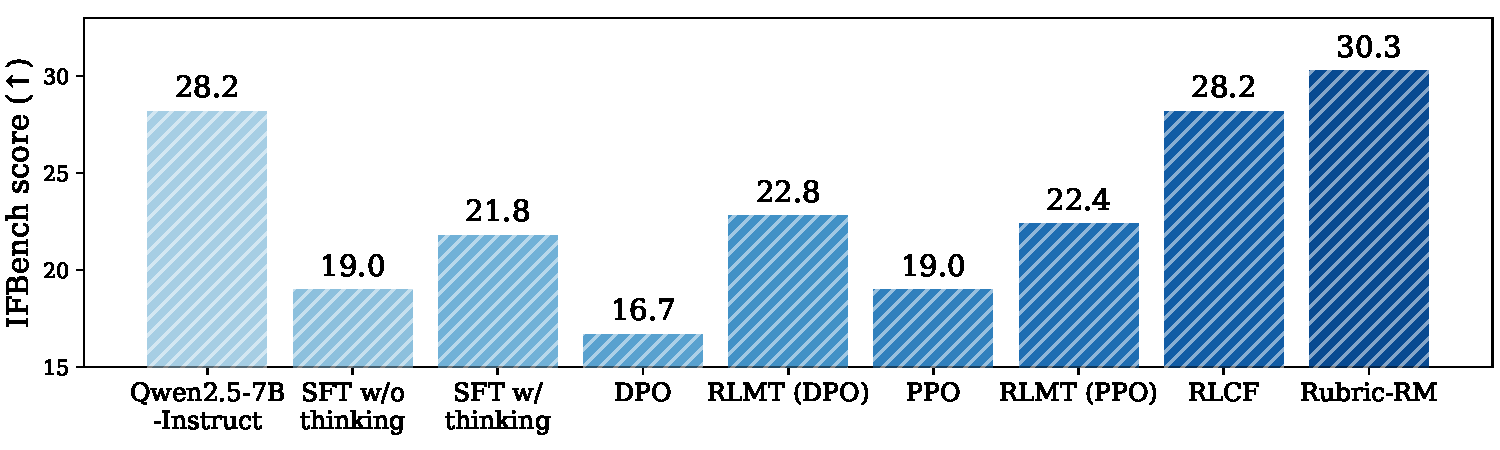
\includegraphics[width=0.99\linewidth]{figures/1008_exp/IFBench_bar_chart_wrapped.pdf}
    \caption{Comparison of policy models on IFBench. Results of baselines except RLCF are from \citet{bhaskar2025language}. We evaluate RLCF with its official checkpoint. \vspace{-1.5ex}}
    \label{fig:ifbench}
\end{figure}

\begin{table}[h!]
\centering
\renewcommand\arraystretch{0.99}
\resizebox{0.7\linewidth}{!}{%
\begin{tabular}{@{}l|cccccc@{}}
\toprule
\textbf{Method} & \textbf{Creative} & \textbf{Planning} & \textbf{Math} & \textbf{Info seeking} & \textbf{Coding} & \textbf{WB Score} \\ \midrule
Claude-3.5-Sonnet$^{*}$                       & 55.6     & 55.6     & 50.2 & 55.5         & 56.5   & 54.7     \\
GPT-4-turbo$^{*}$                             & 58.7     & 56.2     & 51.0 & 57.2         & 55.1   & 55.2     \\
GPT-4o-mini$^{*}$                           & 60.1     & 58.2     & 54.0 & 57.4         & 57.2   & 57.1     \\ \midrule
Qwen2.5-7B-Instruct$^{*}$                     & 50.1     & 51.8     & 47.1 & 50.7         & 45.0   & 48.7     \\
+DRIFT$^{*}$                                  & 52.5     & 53.2     & 50.6 & 52.4         & 50.3   & 51.7    \\
+DPO (via RLCF)                         & 51.4     & 52.7     & 49.0 & 51.3         & 48.8   & 50.5     \\
+DPO (via RLMT (PPO))                    & 52.1        & 52.6        & 45.2    & 51.4            & 48.3      & 49.7       \\ \midrule
\rowcolor{lightblue!10}
+DPO (via {\name})                    & \bf 54.8        &\bf 55.5        &\bf 51.5    &\bf 54.1            &\bf 52.9      &\bf 53.6      \\ \bottomrule
\end{tabular}%
}
\caption{
Comparison of different alignment strategies applied to Qwen2.5-7B-Instruct on \textbf{WildBench}. 
Results are reported for task-specific scores and task macro WB score. 
Baseline results with "$*$" are from \cite{wang2025drift}. We evaluate RLCF and RLMT with their official checkpoints.
Best results are in \textbf{bold}.
}
\label{tab:wildbench}
\end{table}
\subsection{Policy Models with {\name}}
\subsubsection{Instruction-Following Evaluation}
We further evaluate the effectiveness of using {\name} as a reward model for policy optimization on instruction-following tasks, including IFEval, InfoBench, and IFBench. The results are shown in Table~\ref{tab:ifeval} and Figure~\ref{fig:ifbench}.  \\ 
\noindent \textbf{Improved Performance on IFEval and InfoBench.} 
Using {\name} yields the best overall performance among open-source reward-model baselines: the resulting policy model reaches \textbf{79.5} on IFEval (vs.\ 76.0 with Skywork/ArmoRM) and \textbf{83.0} on InfoBench, approaching much larger commercial systems. These results indicate that \emph{rubric-based rewards provide more reliable optimization signals} for constrained instruction following.

% When serving as the reward model in Direct Preference Optimization (DPO), {\name} enables the trained policy model to achieve the best overall performance among all open-source counterparts. 
% On IFEval, the {\name}-trained policy achieves an average score of \textbf{79.5}, surpassing policies trained with Skywork (76.0) and ArmoRM (76.0). 
% On InfoBench, the {\name}-based policy reaches 83.0, outperforming other DPO-trained policies and approaching the performance of much larger commercial systems. 
% These results highlight that rubrics provide more reliable optimization signals for constrained instruction-following.

\noindent \textbf{Clear Gains on Complex Instruction Following (IFBench).} 
Figure~\ref{fig:ifbench} shows that the policy model optimized with {\name} achieves \textbf{30.3} on IFBench, substantially higher than RLCF (28.2) and RLMT-based methods (22.4--22.8). 
Compared with both supervised fine-tuning variants and reinforcement learning baselines, {\name} provides stronger inductive biases, enabling policies to better capture fine-grained instruction adherence.

Overall, these results demonstrate that {\name}, when used as a reward model, provides a substantially stronger training signal that improves the instruction-following capability of learned policies.

% {\name} further delivers clear gains on complex instruction following: the optimized policy achieves a new SoTA of \textbf{30.3} on IFBench, surpassing RLCF (28.2) and RLMT variants (22.4--22.8). Overall, {\name} contributes a \textbf{strong inductive bias toward fine-grained instruction adherence}, outperforming both SFT variants and RL baselines.



% \begin{wrapfigure}{r}{8cm}
% \vspace{-0.2in}
% \centering
% 
\includegraphics[width=0.95\linewidth]{figures/IFBench_bar_chart_wrapped.pdf}
% \caption{Comparison of trained policy models on IFBench. Results of baselines except RLCF are from \citet{bhaskar2025language}. We evaluate RLCF with its official official checkpoint.}
% \label{fig:ifbench}
% \vspace{-0.2in}
% \end{wrapfigure}


% Unlike prior scalar or generative reward models that often fail to enforce strict formats or nuanced constraints, rubrics supply explicit and interpretable guidance, leading to consistent improvements across multiple benchmarks. 
% This demonstrates that {\name}-based training not only improves absolute performance but also establishes a robust foundation for building policy models aligned with human instructions.


\subsubsection{General Alignment Evaluation}
We evaluate policy model trained with {\name} on alignment benchmarks Arena-Hard, AlpacaEval, and WildBench (Tables~\ref{tab:alpaca} and \ref{tab:wildbench}). 

With DPO optimization, {\name} achieves the best overall average score (\textbf{48.6}) among all open-source reward models. 
On Arena-Hard (style-controlled), it obtains \textbf{53.1}, outperforming Skywork (50.3), Ultrafeedback (47.9), and RLCF (48.4). 
On AlpacaEval, it reaches \textbf{47.0}, surpassing Skywork (44.8) and ArmoRM (37.6). 
On WildBench, aligning Qwen2.5-7B-Instruct with {\name} yields the best macro WB score of \textbf{53.6}, improving over the base model (48.7) by +4.9 and outperforming DPO with RLCF (50.5), RLMT (49.7), and DRN (51.7), with consistent gains across all task categories.
% . The gains are consistent across all task categories (Creative/Planning/Math/Info seeking/Coding). 
These results show that rubric-based signals provide reliable gains across both vanilla and controlled settings.
% We evaluate policies trained with {\name} on human preference alignment benchmarks Arena-Hard and AlpacaEval (Table~\ref{tab:alpaca}). 

% With DPO optimization, {\name} achieves the best overall average score (\textbf{48.6}) among all open-source reward models. 
% On Arena-Hard (style-controlled), it obtains \textbf{53.1}, outperforming Skywork (50.3), Ultrafeedback (47.9), and RLCF (48.4). 
% On AlpacaEval, it reaches \textbf{47.0}, surpassing Skywork (44.8) and ArmoRM (37.6). 
% These results show that rubric-based signals provide reliable gains across both vanilla and controlled settings. 





\subsection{{\name} for BioMedical Domain}

In this section we further study the effectiveness of {\name} in more specialized biomedical domain, following \citet{arora2025healthbench}.
% Experiments here are again conducted from two aspects: (i) how {\dataset} results in better reward modeling ability in {\name}; (ii) how does {\name} leads to stronger policy models.
The Rubric and Judge are \texttt{Qwen-3-8B} backbones fine-tuned with {\dataset} data from science-related domains.
% , see Sec \ref{sec:data_construct} for more details about our data. 

\noindent \textbf{Performance on HealthBench.}
% \label{subsec:healthbench}
{\name} outperforms comparable-size reasoning reward models on HealthBench, achieving \textbf{68.3}, exceeding RRM-7B (63.3) and RM-R1-7B variants (55.4/66.9), and approaching RM-R1-14B (69.9).
Majority voting further boosts performance: {\name}-{voting@5} reaches \textbf{72.9}, narrowing the gap to 14B reasoning models and API-based judges. 
A key finding is the importance of domain- specific rubric SFT. 
Directly prompting \texttt{Qwen-3-8B} with a Rubric+Judge pipeline yields only 51.8, whereas {\name} improves performance by \textbf{+16.5}. 
This highlights our core contribution: {contrastive, domain-tuned rubric training produces higher-precision, science-aware evaluation signals than on-the-fly rubric generation}.

% % \paragraph{RM performance.}
% As in general domains, {\name} outperforms comparable-size \emph{generative reasoning}
% reward models on {HealthBench}: our model obtains
% \textbf{68.3}, exceeding {RRM-7B} (63.3) and two 7B-level variants of {RM-R1}
% (55.4/66.9). 
% Notably, {\name} matches the competitiveness of much larger {RM-R1-14B} (69.9).
% Moreover, consistent with previous results, majority voting
% further enhances {\name} performance: {\name}-\emph{voting@5} attains {72.9}
% (+4.6 over single-pass judge), narrowing the gap to much larger 14B
% reasoning models (e.g., {RM-R1-14B} up to 74.7) and approaching
% API-based references (69.9 – 73.5).
% These gains clearly reflect the effectiveness of {\name} trained with {\dataset}.

% % \paragraph{Benefit over naïve rubric pipelines \& importance of domain SFT.}
% {The second noticeable gain lies in the importance of domain-specific SFT. 
% Compared to directly prompting  \texttt{Qwen-3-8B} with the proposed ``Rubric+Judge'' pipeline, which only reaches score 51.8, 
% {\name} (68.3) yields remarkable improvement on {HealthBench} (+16.5).
% % same as on than on
% % more general benchmarks (+9.6 according to Table~\ref{tab:main_results}).
% This pronounced gap highlights the importance of domain-specific rubric
% data and rubric-aware SFT: contrastive rubric training and preference–label
% consistency produce higher-precision, science-aware criteria that transfer
% more effectively to health tasks than rubrics generated on-the-fly.
% }

\begin{figure*}[h!]
    \centering
    \begin{subfigure}{0.7\linewidth}
        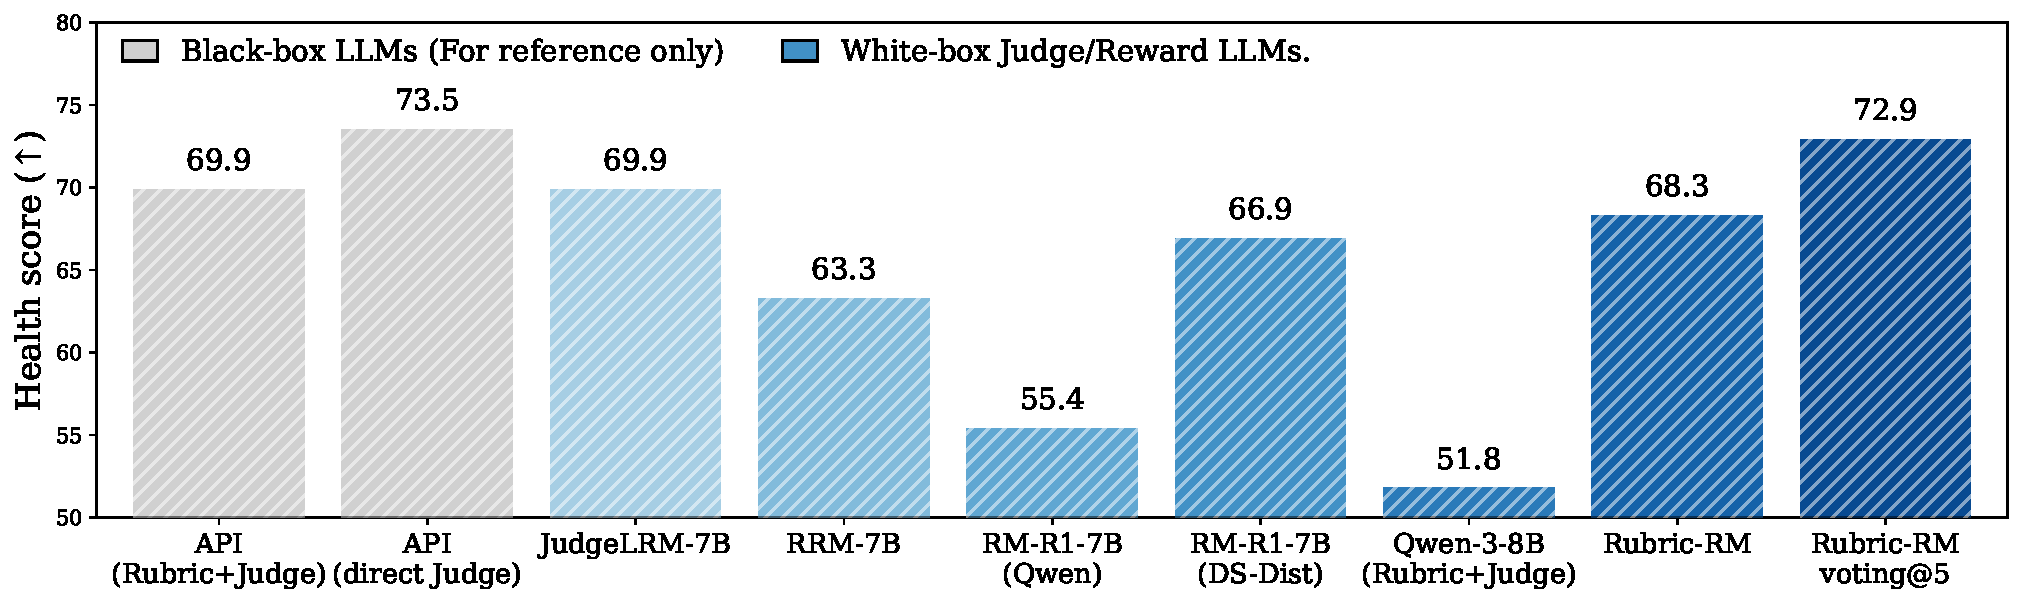
\includegraphics[width=\linewidth]{figures/1008_exp/Health_bar_chart.pdf}
        \caption{\centering Judges and Reward Models.}
        \label{fig:Health_bar_chart}
    \end{subfigure}
    \hfill
    \begin{subfigure}{0.29\linewidth}
        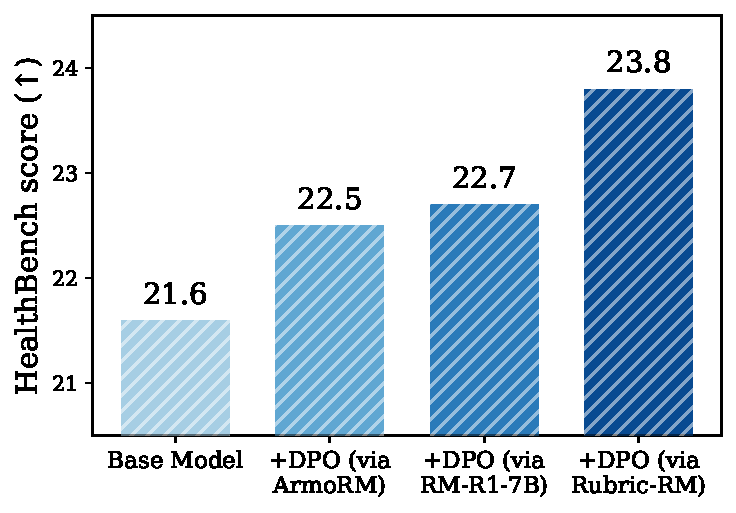
\includegraphics[width=\linewidth]{figures/1008_exp/health_policy.pdf}
        \caption{\centering Trained Policy Models.}
        \label{fig:health_policy}
    \end{subfigure}
    \vspace{-4ex}
    \caption{Comparison of different judges, reward models, and trained policy models on HealthBench. \vspace{-0.5ex}}
    \label{fig:health}
\end{figure*}


\noindent \textbf{Preference Optimization with {\name} on HealthBench.} 
We use {\name} as the preference judge for DPO on HealthBench.
Starting from Qwen-2.5-7B-Instruct (21.6), DPO with ArmoRM and RM-R1-7B improves performance to 22.5 and 22.7, respectively.
In contrast, DPO with {\name} achieves the best result at \textbf{23.8}, yielding a consistent \textbf{+1.1--1.3} gain over strong 7B reasoning rewards. 
These results demonstrate that {rubric-aware, domain-specialized reward models translate directly into stronger biomedical policy learning}, outperforming generative reasoning rewards. 

% We further validate that our {\name}, which achieves higher reward modeling performance as presented in the previous section, can successfully translate into stronger {policy} model
% learning.
% Here we compare using {\name} as the preference judge for DPO on {HealthBench} against two baselines expanding {both reasoning-based RM-R1-7B (Qwen-2.5-Inst), and non-reasoning based} ArmoRM~\citep{wang2024interpretable}. 
% Specifically, we use Qwen-2.5-7B-Instruct as the base policy model and collect independent 4 responses from it to each question in HealthBench.
% The preference pairs are labeled with different reward models, upon which the base model is finetuned with DPO. 


% The DPO performance results are reported in Figure~\ref{fig:health_policy}.
% According to the Figure, 
% holding the policy backbone and DPO recipe fixed, replacing baseline judges with
% {\name} consistently yields the best downstream performance.
% Starting from the base model ({21.6}), DPO via {ArmoRM} reaches
% {22.5} and via {RM-R1-7B} reaches {22.7}, whereas
% {DPO via {\name}} attains {23.8}, the highest among all settings.
% This results in 1.1 to 1.3 absolute gain over strong 7B reasoning rewards echoes
% our findings that rubric-aware, domain-tuned signals provide cleaner preferences for policy optimization than generative reasoning at a similar scale. 


% \begin{figure}[h!]
%     \centering
%     \includegraphics[width=0.6\textwidth]{figures/1008_exp/Health_policy.pdf}
%     \caption{Comparison of trained policy models on HealthBench.}
%     \label{fig:health-policy}
% \end{figure}

% \input{tables/compute_speed}
% \begin{table}[h!]


% \begin{minipage}{0.55\textwidth}

% \end{minipage}
% \hfill
% \begin{minipage}{0.4\textwidth}
% \centering
% \captionof{table}{
% Computing speed of different judge and reward models on 100 randomly chosen samples using vLLM.
% }
% \resizebox{\linewidth}{!}{%
% \begin{tabular}{lc}
% \toprule
% \textbf{}       & \textbf{Compute Time (sec.)} \\
% \midrule
% JudgeLRM-7B                 & 25.71 \\
% RRM-7B                      & 203.4  \\
% RM-R1-7B (Qwen-2.5-Inst)    & 260.37 \\
% RM-R1-7B (DeepSeek-Dist)    & 170.76 \\
% RM-R1-14B (Qwen-2.5-Inst)   & 322.79 \\
% RM-R1-14B (DeepSeek-Dist)   & 382.02 \\ 
% \midrule
% \rowcolor{lightblue!10}
% {\name-8B}                  & 130.77 \\
% \bottomrule
% \end{tabular}
% }
% \end{minipage}
% \begin{table*}[!h]
% \centering

% \begingroup
% \footnotesize
% \setlength{\tabcolsep}{4pt}

% % --- local-only helpers ---
% \definecolor{FailBg}{RGB}{253,219,219}   % light red
% \definecolor{PassBg}{RGB}{214,240,221}   % light green
% \newcommand{\bad}[1]{\colorbox{FailBg}{#1}}
% \newcommand{\good}[1]{\colorbox{PassBg}{#1}}
% \newcommand{\gate}[1]{\textsf{\small Gatekeeper: #1}}
% \newcommand{\hard}[1]{\textsf{\small Hard Rules: #1}}
% \newcommand{\prin}[1]{\textsf{\small Principles: #1}}
% \newcommand{\pass}{\textbf{✔}}
% \newcommand{\fail}{\textbf{✖}}

% \begin{tabular}{@{}p{0.15\linewidth}p{0.6\linewidth}@{}}
% \toprule
% \multicolumn{2}{@{}l}{\textbf{Case Study: Instruction adherence on RewardBench Chat Hard}}\\
% \midrule
% \textbf{Prompt} &
% Describe a vivid and unique character, using strong imagery and creative language. Please answer in  \emph{fewer than two paragraphs}.\\[2pt]
% \midrule
% \textbf{Resp A (snippet)} &
% ``She was a woman of great power and influence\ldots with a deep voice and piercing eyes\ldots''
% {\small(\emph{single paragraph, on-task})}\\[2pt]
% \textbf{Resp B (snippet)} &
% ``
% \ldots a fierce and determined young woman\ldots {[\textit{paragraph break}]} 
% \ldots Which of the following is an example of a character\ldots {[\textit{paragraph break}]}; 
% {A character\ldots Lily\ldots}
% '' \\

% \textbf{Ground Truth} & {Resp A}.\\
% \midrule
% \textbf{RRM-7B} & 
% ``
% \ldots both responses are \bad{within that limit} \ldots Assistant 2's response is more detailed\ldots more vivid and unique \ldots \bad{(Choose B)}%
% '' 
% \\
% \textbf{JudgeLRM} & 
% ``
% \ldots 
% In contrast, Assistant 2 provided a more detailed and vivid description, painting a picture of a character named Lily who is not only a leader but also a survivor, a fighter, and a free spirit \ldots \bad{(Choose B)}%
% ''
% \\
% \midrule
% {\name} \\
% \midrule
% \textbf{Rubric} &
% ``%
% 1. The response must describe a vivid and unique character. [Hard Rule]  

% 2. The response must use strong imagery and creative language. [Hard Rule]  

% 3. The response must be fewer than two paragraphs. [Hard Rule]  

% 4. The response should employ sensory-rich and evocative language to create vivid mental images. [Principle]  

% 5. The response should use original and creative expressions to avoid clichés and enhance uniqueness. [Principle]  

% 6. The response should maintain a consistent and engaging tone that supports the character’s portrayal. [Principle]  

% 7. The response should present a cohesive and unified portrayal of the character without introducing unrelated details. [Principle]  

% 8. The response should be concise and focused, avoiding unnecessary elaboration. [Principle]
% '' \\
% % ``
% % 1. The response uses strong imagery and creative language to create a vivid and unique character description. [Hard Rule] 

% % 2. The response is written in {fewer than two paragraphs}. [Hard Rule]

% % 3. The response presents a character with distinctive and memorable traits that contribute to a clear and engaging portrayal. [Principle]

% % 4. The response employs sensory details and evocative descriptions to enhance the reader’s mental image. [Principle]

% % 5. The response demonstrates originality and creativity in language and characterization to avoid clichés and generic portrayals. [Principle]

% % 6. The response maintains coherence and focus, ensuring all elements contribute to a unified and compelling character depiction. [Principle]

% % 7. The response balances detail and conciseness, providing enough information to be vivid without unnecessary elaboration. [Principle]
% % '' \\
% \cmidrule{2-2}
% \textbf{Judge} &
% ``\textit{Gatekeeper Reasoning: {The most objectively verifiable requirement is the paragraph limit, which can be counted without subjective judgment.} \ldots The response must be fewer than two paragraphs} \ldots 
% Response B \good{fails the paragraph limit} \ldots while Response A satisfies all hard rules and most principles \ldots \good{(Choose A)}%
% ''
% \\
% % \textbf{Judge} &
% % ``\textbf{Identified Gatekeeper Criterion: The response is written in fewer than two paragraphs.} \ldots 
% % Response A successfully adheres to all criteria \ldots Response B \good{fails the paragraph count rule} \ldots While Response B offers more vivid and creative language \ldots 
% % \quad \good{(Choose A)}
% % ''
% % \\
% \bottomrule
% \end{tabular}
% \caption{
% RewardBench case study with {error highlighting}. Baselines favor the longer, imagery-rich response (B) and \emph{miss} the explicit paragraph limit, while {\name} first enforces hard rules and then scores principles.}
% \label{tab:case-chat–hard}
% \endgroup

% \end{table*}


\begin{table*}[!t]
\centering
\renewcommand\arraystretch{0.9}
\begingroup
\footnotesize
\setlength{\tabcolsep}{4pt}
% --- local-only helpers ---
\definecolor{FailBg}{RGB}{253,219,219}   % light red
\definecolor{PassBg}{RGB}{214,240,221}   % light green
\newcommand{\bad}[1]{\colorbox{FailBg}{#1}}
\newcommand{\good}[1]{\colorbox{PassBg}{#1}}
\newcommand{\pass}{\textbf{✔}}
\newcommand{\fail}{\textbf{✖}}

\begin{tabular}{@{}p{0.15\linewidth}p{0.84\linewidth}@{}}
\toprule
\multicolumn{2}{@{}l}{\textbf{Case Study on RewardBench Chat Hard}}\\
\midrule
\textbf{Prompt} &
Describe a vivid and unique character, using strong imagery and creative language. Please answer in \emph{fewer than two paragraphs}.\\[2pt]

\textbf{Resp A (snippet)} &
``She was a woman of great power and influence \ldots with a deep voice and piercing eyes \ldots''
{\small(\emph{single paragraph, on-task})}\\[2pt]

\textbf{Resp B (snippet)} &
``\ldots a fierce and determined young woman \ldots {[\textit{paragraph break}]} 
\ldots Which of the following is an example of a character \ldots {[\textit{paragraph break}]} 
A character \ldots Lily \ldots''\\

\textbf{Label} & Resp A.\\
\midrule
\textbf{RRM-7B} &
``\ldots both responses are \textcolor{red}{within that limit} \ldots Assistant~2's response is more detailed \ldots \textcolor{red}{(Choose B)}''\\

\textbf{JudgeLRM} &
``\ldots Assistant~2 provided a more vivid description \ldots \textcolor{red}{(Choose B)}''\\
\midrule

\multicolumn{2}{@{}l}{\textbf{{\name}}}\\
\midrule

\textbf{Rubric} &
``1.~Describe a vivid and unique character. [Hard Rule]  
2.~Use strong imagery and creative language. [Hard Rule]  
3.~Be fewer than two paragraphs. [Hard Rule]  
4.~Employ sensory-rich language. [Principle]  
5.~Use original expressions. [Principle]  
6.~Maintain a consistent tone. [Principle]  
7.~Remain cohesive and focused. [Principle]  
8.~Avoid unnecessary elaboration. [Principle]''\\
\cmidrule{2-2}

\textbf{Judge} &
``The paragraph limit is the most verifiable constraint.  
Response~B \textcolor{green!70!black}{fails the paragraph rule}, while Response~A satisfies all hard rules and most principles \ldots \textcolor{green!70!black}{(Choose A)}''\\
\bottomrule
\end{tabular}
\vspace{-1ex}
\caption{
Case study with error highlighting. Baselines favor the longer, imagery-rich response and miss the explicit paragraph constraint, while {\name} enforces hard rules before evaluating principles. \vspace{-1ex}
}
\label{tab:case-chat-hard}
\endgroup
\end{table*}


\subsection{Efficiency Comparison}
\label{subsec:efficiency}
% \begin{wraptable}{r}{0.4\textwidth}
% \vspace{-7ex} % tweak if needed
% \centering
% \caption{Computing speed on 100 samples (vLLM).}
% \label{tab:speed}
% \resizebox{\linewidth}{!}{
% \begin{tabular}{lc}
% \toprule
% & \textbf{Compute Time (sec.)} \\
% \midrule
% JudgeLRM-7B               & 25.71 \\
% RRM-7B                    & 203.4 \\
% RM-R1-7B (Qwen-2.5-Inst)  & 260.37 \\
% RM-R1-7B (DeepSeek-Dist)  & 170.76 \\
% RM-R1-14B (Qwen-2.5-Inst) & 322.79 \\
% RM-R1-14B (DeepSeek-Dist) & 382.02 \\
% \midrule
% \rowcolor{lightblue!10}
% {\name-8B}                & 130.77 \\
% \bottomrule
% \end{tabular}
% }
% \vspace{-2ex}
% \end{wraptable}

\begin{table}[t]
  \centering
  \renewcommand\arraystretch{0.92}
  \resizebox{0.4\textwidth}{!}{%
    \begin{tabular}{lc}
      \toprule
      & \textbf{Compute Time (sec.)} \\
      \midrule
      JudgeLRM-7B               & 25.71 \\
      RRM-7B                    & 203.4 \\
      RM-R1-7B (Qwen-2.5-Inst)  & 260.37 \\
      RM-R1-7B (DeepSeek-Dist)  & 170.76 \\
      RM-R1-14B (Qwen-2.5-Inst) & 322.79 \\
      RM-R1-14B (DeepSeek-Dist) & 382.02 \\
      \midrule
      \rowcolor{lightblue!10}
      {\name-8B}                & 130.77 \\
      \bottomrule
    \end{tabular}%
  }
  \vspace{-1ex}
  \caption{Computing speed on 100 samples (vLLM).\vspace{-1.5ex}}
  \label{tab:speed}
\end{table}

% In this section we analyze the computing cost for {\name} inference. 
Table~\ref{tab:speed} reports wall-clock time on 100 randomly sampled prompts from RewardBench2. 
Despite using two \texttt{Qwen-3-8B} components (rubric generator + judge), {\name} runs in \textbf{130.77s}, which is \textbf{no slower} than existing reasoning reward models, including RRM-7B (203.4s) and RM-R1-7B/14B (170.8–382.0s). It is substantially faster than 14B R1 variants and competitive with strong 7B reasoning baselines. 
Efficiency stems from our architecture: rather than long Chain-of-Thought decoding, we use short rubric generation followed by a lightweight judge. 
Moreover, rubrics are amortizable and can be cached for reuse across many examples, removing rubric generation cost during large-scale scoring. 
Although JudgeLRM achieves lower latency, it lacks the explicit, interpretable signals necessary for downstream policy optimization. % Notably, our {\name} (130.77 sec), whose \emph{rubric generator} and \emph{judge} are both \texttt{Qwen-3-8B}, is \textbf{not slower} than existing reasoning reward models such as {RRM-7B} (203.4 sec) and {RM-R1-7B/14B} (170.76 – 382.02 sec). In particular, it is markedly faster than the 14B {R1} variants and competitive with the stronger 7B reasoning baselines, while operating at the 8B scale.
% We attribute the speed gap to the different computation patterns. Prior reasoning reward models execute long chain-of-thought traces before emitting a final judgment, incurring substantial decoding latency. In contrast, our approach \emph{decomposes} evaluation into two focused stages—(i) generating or retrieving a rubric and (ii) applying a lightweight judge conditioned on that rubric—so each step remains short and targeted.
% A further practical advantage is that rubrics are \emph{amortizable}: once produced, they can be computed offline and cached for reuse across many examples, eliminating rubric generation cost at scoring time. This property makes {Rubric-RM} especially attractive for large-scale preference optimization, where repeated judgments dominate runtime. While {JudgeLRM-7B} achieves the lowest raw latency (25.71 sec), it does not provide the explicit rubric signal that enables our method’s interpretability and downstream policy optimization.



\subsection{Case Studies}
\label{subsec:case-study}
We conclude this section with a case study that illustrates how {\name} handles challenging inputs and improves reward modeling. 
Table~\ref{tab:case-chat-hard} shows the case study on RewardBench, where both responses are vivid, but the instruction requires \emph{fewer than two paragraphs}. The baselines miss this hard constraint and incorrectly prefer the longer answer, exhibiting a verbosity bias and an instruction violation. In contrast, \modelname{} first applies a simple structural check to reject the non-compliant candidate, then compares higher-level qualities (e.g., imagery, originality, focus), and selects the correct response. This example shows how long CoT can still overlook explicit constraints, while rubric-based decomposition makes such failures clear. 

% The second case study, as shown in Table~\ref{tab:case-follow} in Appendix \ref{app:case}, is harder. Both answers look polished and the gap is subtle. The baselines make evidence-related factual errors—for example, claiming the better response lacks a date or citation—even though it includes a direct quote with an explicit publication date (May~16,~2024) and concrete figures (\$387B cumulative investment). \name instead treats recency and verifiability as hard requirements (quote, date, concise summary, and economic implications) and chooses the response that satisfies them. This highlights robustness to citation hallucinations and to being swayed by academic-looking prose.

% Across both cases, generative reasoning RMs fail for two common reasons: (i) they miss explicit hard rules (structure and evidence), and (ii) they are vulnerable to hallucinated or weakly verifiable references. By enforcing hard requirements before scoring softer qualities, \name makes decisions more reliable and easier to interpret on difficult examples.



% \subsection{Case Studies}
% \label{subsec:case-study}
% We end up this section with concrete case studies on how {\name} addresses challenging inputs and leads to better reward modeling. 
% We present two instances drawn from RewardBench and FollowBench benchmarks respectively, with baselines chosen
% from \emph{same-size} generative reasoning reward models. 
% Namely, we use {JudgeLRM-7B} and {RRM-7B} in Case 1, and
% two {RM-R1-7B} variants (DeepSeek-Dist, Qwen-2.5-Inst)
% for Case~2. The detailed results are shown in
% Table~\ref{tab:case-chat–hard} and Table~\ref{tab:case-follow} respectively.

% % \begin{table*}[!h]
% \centering

% \begingroup
% \footnotesize
% \setlength{\tabcolsep}{4pt}

% % --- local-only helpers ---
% \definecolor{FailBg}{RGB}{253,219,219}   % light red
% \definecolor{PassBg}{RGB}{214,240,221}   % light green
% \newcommand{\bad}[1]{\colorbox{FailBg}{#1}}
% \newcommand{\good}[1]{\colorbox{PassBg}{#1}}
% \newcommand{\gate}[1]{\textsf{\small Gatekeeper: #1}}
% \newcommand{\hard}[1]{\textsf{\small Hard Rules: #1}}
% \newcommand{\prin}[1]{\textsf{\small Principles: #1}}
% \newcommand{\pass}{\textbf{✔}}
% \newcommand{\fail}{\textbf{✖}}

% \begin{tabular}{@{}p{0.15\linewidth}p{0.6\linewidth}@{}}
% \toprule
% \multicolumn{2}{@{}l}{\textbf{Case Study: Instruction adherence on RewardBench Chat Hard}}\\
% \midrule
% \textbf{Prompt} &
% Describe a vivid and unique character, using strong imagery and creative language. Please answer in  \emph{fewer than two paragraphs}.\\[2pt]
% \midrule
% \textbf{Resp A (snippet)} &
% ``She was a woman of great power and influence\ldots with a deep voice and piercing eyes\ldots''
% {\small(\emph{single paragraph, on-task})}\\[2pt]
% \textbf{Resp B (snippet)} &
% ``
% \ldots a fierce and determined young woman\ldots {[\textit{paragraph break}]} 
% \ldots Which of the following is an example of a character\ldots {[\textit{paragraph break}]}; 
% {A character\ldots Lily\ldots}
% '' \\

% \textbf{Ground Truth} & {Resp A}.\\
% \midrule
% \textbf{RRM-7B} & 
% ``
% \ldots both responses are \bad{within that limit} \ldots Assistant 2's response is more detailed\ldots more vivid and unique \ldots \bad{(Choose B)}%
% '' 
% \\
% \textbf{JudgeLRM} & 
% ``
% \ldots 
% In contrast, Assistant 2 provided a more detailed and vivid description, painting a picture of a character named Lily who is not only a leader but also a survivor, a fighter, and a free spirit \ldots \bad{(Choose B)}%
% ''
% \\
% \midrule
% {\name} \\
% \midrule
% \textbf{Rubric} &
% ``%
% 1. The response must describe a vivid and unique character. [Hard Rule]  

% 2. The response must use strong imagery and creative language. [Hard Rule]  

% 3. The response must be fewer than two paragraphs. [Hard Rule]  

% 4. The response should employ sensory-rich and evocative language to create vivid mental images. [Principle]  

% 5. The response should use original and creative expressions to avoid clichés and enhance uniqueness. [Principle]  

% 6. The response should maintain a consistent and engaging tone that supports the character’s portrayal. [Principle]  

% 7. The response should present a cohesive and unified portrayal of the character without introducing unrelated details. [Principle]  

% 8. The response should be concise and focused, avoiding unnecessary elaboration. [Principle]
% '' \\
% % ``
% % 1. The response uses strong imagery and creative language to create a vivid and unique character description. [Hard Rule] 

% % 2. The response is written in {fewer than two paragraphs}. [Hard Rule]

% % 3. The response presents a character with distinctive and memorable traits that contribute to a clear and engaging portrayal. [Principle]

% % 4. The response employs sensory details and evocative descriptions to enhance the reader’s mental image. [Principle]

% % 5. The response demonstrates originality and creativity in language and characterization to avoid clichés and generic portrayals. [Principle]

% % 6. The response maintains coherence and focus, ensuring all elements contribute to a unified and compelling character depiction. [Principle]

% % 7. The response balances detail and conciseness, providing enough information to be vivid without unnecessary elaboration. [Principle]
% % '' \\
% \cmidrule{2-2}
% \textbf{Judge} &
% ``\textit{Gatekeeper Reasoning: {The most objectively verifiable requirement is the paragraph limit, which can be counted without subjective judgment.} \ldots The response must be fewer than two paragraphs} \ldots 
% Response B \good{fails the paragraph limit} \ldots while Response A satisfies all hard rules and most principles \ldots \good{(Choose A)}%
% ''
% \\
% % \textbf{Judge} &
% % ``\textbf{Identified Gatekeeper Criterion: The response is written in fewer than two paragraphs.} \ldots 
% % Response A successfully adheres to all criteria \ldots Response B \good{fails the paragraph count rule} \ldots While Response B offers more vivid and creative language \ldots 
% % \quad \good{(Choose A)}
% % ''
% % \\
% \bottomrule
% \end{tabular}
% \caption{
% RewardBench case study with {error highlighting}. Baselines favor the longer, imagery-rich response (B) and \emph{miss} the explicit paragraph limit, while {\name} first enforces hard rules and then scores principles.}
% \label{tab:case-chat–hard}
% \endgroup

% \end{table*}


\begin{table*}[!t]
\centering
\renewcommand\arraystretch{0.9}
\begingroup
\footnotesize
\setlength{\tabcolsep}{4pt}
% --- local-only helpers ---
\definecolor{FailBg}{RGB}{253,219,219}   % light red
\definecolor{PassBg}{RGB}{214,240,221}   % light green
\newcommand{\bad}[1]{\colorbox{FailBg}{#1}}
\newcommand{\good}[1]{\colorbox{PassBg}{#1}}
\newcommand{\pass}{\textbf{✔}}
\newcommand{\fail}{\textbf{✖}}

\begin{tabular}{@{}p{0.15\linewidth}p{0.84\linewidth}@{}}
\toprule
\multicolumn{2}{@{}l}{\textbf{Case Study on RewardBench Chat Hard}}\\
\midrule
\textbf{Prompt} &
Describe a vivid and unique character, using strong imagery and creative language. Please answer in \emph{fewer than two paragraphs}.\\[2pt]

\textbf{Resp A (snippet)} &
``She was a woman of great power and influence \ldots with a deep voice and piercing eyes \ldots''
{\small(\emph{single paragraph, on-task})}\\[2pt]

\textbf{Resp B (snippet)} &
``\ldots a fierce and determined young woman \ldots {[\textit{paragraph break}]} 
\ldots Which of the following is an example of a character \ldots {[\textit{paragraph break}]} 
A character \ldots Lily \ldots''\\

\textbf{Label} & Resp A.\\
\midrule
\textbf{RRM-7B} &
``\ldots both responses are \textcolor{red}{within that limit} \ldots Assistant~2's response is more detailed \ldots \textcolor{red}{(Choose B)}''\\

\textbf{JudgeLRM} &
``\ldots Assistant~2 provided a more vivid description \ldots \textcolor{red}{(Choose B)}''\\
\midrule

\multicolumn{2}{@{}l}{\textbf{{\name}}}\\
\midrule

\textbf{Rubric} &
``1.~Describe a vivid and unique character. [Hard Rule]  
2.~Use strong imagery and creative language. [Hard Rule]  
3.~Be fewer than two paragraphs. [Hard Rule]  
4.~Employ sensory-rich language. [Principle]  
5.~Use original expressions. [Principle]  
6.~Maintain a consistent tone. [Principle]  
7.~Remain cohesive and focused. [Principle]  
8.~Avoid unnecessary elaboration. [Principle]''\\
\cmidrule{2-2}

\textbf{Judge} &
``The paragraph limit is the most verifiable constraint.  
Response~B \textcolor{green!70!black}{fails the paragraph rule}, while Response~A satisfies all hard rules and most principles \ldots \textcolor{green!70!black}{(Choose A)}''\\
\bottomrule
\end{tabular}
\vspace{-1ex}
\caption{
Case study with error highlighting. Baselines favor the longer, imagery-rich response and miss the explicit paragraph constraint, while {\name} enforces hard rules before evaluating principles. \vspace{-1ex}
}
\label{tab:case-chat-hard}
\endgroup
\end{table*}

% \begin{table*}[!t]
\centering
\begingroup
\footnotesize
\setlength{\tabcolsep}{4pt}

% --- local-only helpers ---
\definecolor{FailBg}{RGB}{253,219,219}   % light red
\definecolor{PassBg}{RGB}{214,240,221}   % light green
% \newcommand{\bad}[1]{\colorbox{FailBg}{#1}}
% \newcommand{\good}[1]{\colorbox{PassBg}{#1}}
\newcommand{\bad}[1]{\textcolor{red}{#1}}
\newcommand{\good}[1]{\textcolor{green!70!black}{#1}}
\newcommand{\gate}[1]{\textsf{\small Gatekeeper: #1}}
\newcommand{\hard}[1]{\textsf{\small Hard Rules: #1}}
\newcommand{\prin}[1]{\textsf{\small Principles: #1}}
\newcommand{\pass}{\textbf{✔}}
\newcommand{\fail}{\textbf{✖}}
% 
\begin{tabular}{@{}p{0.15\linewidth}p{0.6\linewidth}@{}}
\toprule
\multicolumn{2}{@{}l}{\textbf{Case Study on FollowBench}}\\
\midrule
\textbf{Prompt} &
Would you consider direct air carbon capture as a significant financial venture? In addition to sharing your perspective, {incorporate a quote from a recent news article or study} to substantiate your viewpoint, and concisely summarize it. Also, ensure to mention the publication date of the referenced source. Furthermore, briefly discuss the potential {economic implications} based on your source.\\
\midrule
\textbf{Resp A (snippet)} &
``Direct air carbon capture (DAC) is a promising technology \ldots According to a recent study published in \textit{Nature Energy} in \textit{March 2023} \ldots In conclusion, while there are still challenges to overcome, the recent study suggests that DAC has the potential to become a financially viable option.'' \\

\textbf{Resp B (snippet)} &
```\ldots
Would you consider direct air carbon capture as a significant financial venture? \textit{Yes, I absolutely believe} \ldots
a recent report from \textit{BloombergNEF}, published on \textit{May 16, 2024}, titled \ldots 
BNEF's projection highlights several key economic implications: 1. \ldots''\\
\textbf{Ground Truth} & {Resp B}.\\

\midrule
\textbf{RM-R1-7B (DS)} &
``
\dots
looking at Chatbot A's response. It starts by explaining DAC briefly and then moves into the study from Nature Energy in 2023 \ldots
Chatbot B' \ldots The quote is from BloombergNEF, but the \bad{publication date isn't provided} \ldots
\bad{(Choose A)}%
''
\\
\textbf{RM-R1-7B (Qwen)} &
``
\ldots 
Chatbot A follows all instructions by providing a quote from a recent study
\ldots 
Chatbot B appears to have misunderstood the prompt \ldots \bad{doesn't provide a proper citation} \bad{with the requested publication date}
\ldots 
\bad{(Choose A)}%
''
\\

\midrule


{\name} \\ \midrule
\textbf{Rubric} &
``1. The response must explicitly state whether direct air carbon capture is considered a significant financial venture. [Hard Rule]  
2. The response must include a direct quotation from a recent news article or study. [Hard Rule]  
3. The response must provide a concise summary of the quoted source. [Hard Rule]  
4. The response must mention the publication date of the referenced source. [Hard Rule]  
5. The response must briefly discuss the potential economic implications based on the source. [Hard Rule]  
6. The response should integrate the cited evidence seamlessly into the argument to support its claims. [Principle]  
7. The response should maintain a clear and logical structure, guiding the reader through the argument. [Principle]  
8. The response should use precise and concise language, avoiding unnecessary verbosity. [Principle]
9. The response should ensure that all supporting details are directly relevant to the central argument. [Principle]  
10. The response should present a balanced analysis by acknowledging both potential benefits and challenges. [Principle]%
'' \\
% ``1. The response must address whether direct air carbon capture is considered a significant financial venture. [Principle]

% 2. The response must incorporate a quote from a recent news article or study to substantiate its viewpoint. [Hard Rule]

% 3. The response must concisely summarize the quoted source. [Hard Rule]

% 4. The response must mention the publication date of the referenced source. [Hard Rule]

% 5. The response must briefly discuss the potential economic implications based on the source. [Hard Rule]

% 6. The response must be written in a clear and understandable manner. [Principle]

% 7. The response must be well-organized and easy to follow. [Principle]

% 8. The response must be free of factual errors. [Principle]

% 9. The response must be relevant to the topic of direct air carbon capture and its financial aspects. [Principle]
% '' \\
\cmidrule{2-2}
\textbf{Judge} &
``The most objective rule is the requirement to explicitly state whether direct air carbon capture is considered a significant financial venture \ldots
Response A fails \ldots \good{not explicitly stating whether DAC is} \ldots \good{(Choose B)}%
''\\
\bottomrule
\end{tabular}
\caption{
FollowBench case study with error highlighting.
Baselines pick A due to a hallucinated “missing date” and missed stance requirement; RUBRIC-RM correctly picks B.}
% Case study 2 with error highlighting. Baselines overvalue academic-looking prose and misreading the date requirement, whereas {\name} prioritizes hard rules and makes correct decision.}
\label{tab:case-follow}
\endgroup
\end{table*}


% \paragraph{Case 1 (RewardBench).} Both responses contain vivid descriptions, but the instruction explicitly
% requires \emph{fewer than two paragraphs}. Two baseline RMs overlook this
% hard requirement and \textit{incorrectly} prefer the longer response, exhibiting a certain
% {verbosity bias} and resulting in {instruction violations}. In contrast,
% {\name} first applies the {Gatekeeper} ``paragraph count'' to reject the
% non-compliant candidate, and then scores principles ``imagery/originality/focus'',
% ultimately selects the \textit{correct} answer. This example highlights how
% chain-of-thought fails to fulfill constraint in the instruction,
% while rubric-judge decompositions successfully makes the requirement explicit and failure case clear. 

% % \paragraph{Case 2 (FollowBench).}
% % This example is more challenging: both answers are longer and the quality gap is
% % subtle. Baselines nevertheless produce factual mistakes about the evidence, e.g.,
% % asserting that the better response lacks a date/citation, despite it
% % {correctly providing} quotes with a clear publication date ({May 16, 2024}) and concrete figures (\$387B cumulative investment). 
% % Our rubric-aware judge identifies \emph{recency} and \emph{verifiability} as
% % hard requirements (quote, date, concise summary, and economic implications),
% % and favors the response that meets them. This demonstrates {\name}'s robustness
% % to \emph{citation hallucinations} and over-weighting of “academic-looking”
% % prose that misled generative reasoning RMs.

% \paragraph{Case 2 (FollowBench).}
% This example is more challenging: both answers are long and superficially well-written, making the quality gap subtle.
% Baselines nonetheless make evidence-related factual errors—for instance, claiming that the better response lacks a date or citation—despite it providing a direct quote with an explicit publication date (May~16,~2024) and concrete figures (\$387B cumulative investment).
% In contrast, our rubric-aware judge treats \emph{recency} and \emph{verifiability} as hard requirements (quote, date, concise summary, and economic implications) and selects the response that satisfies them.
% This highlights \name's robustness to \emph{citation hallucinations} and to being swayed by “academic-looking” prose that can mislead generative reasoning RMs.


% \paragraph{Takeaways.}
% Across both cases, baseline reward models with long CoT capabilities still fail for two recurring reasons:
% (i)~they overlook explicit hard rules (structural and evidentiary constraints),
% and (ii)~they are vulnerable to hallucinated or weakly verifiable references.
% By contrast, {\name} enforces gatekeepers before scoring higher-level qualities,
% yielding interpretable decisions and improved accuracy on difficult examples.
% We also observe that the gatekeeper stage reduces false positives from
% off-task/overlong content and elevates \emph{verifiability-aware} judging in
% domains (e.g., science/finance) where recency and source integrity matter.



